\subsection{Secure Group Communication}
The most simple approach to this challange is to create a secret \textit{group key} (\ac{GK}) each time multible devices need to access the same file. This schemes are called "Secure Group Communication" (\ac{SGC}). The main idea is to reduce the number of filekeys by encrypting all the files with a unique \ac{GK} that is only known to the members in the share. Very simple approaches use a so called \textit{Key Distribution Center} (\ac{KDC}) to distribute the group keys to each member. However, while Bdrive could manage forward secrecy quite easily, this schemes suffer from additional rekeying overhead if a member leaves the group. 

% Mutlicast in group communications
Often Secure Group Communications are mentioned together with \textit{multicat messages}. The idea is that on \textit{unicast} a central authority is required that manages authentication and authorization to decide which entity should access which content. With multicast messsages content is distributed to each entity regardless if this entity is authorized to view the content. Authorization is handled via encryption of the content. If an entity owns the key to decrypt the data it is implizity authorized to view the content. Multicast messages are expecially handy in group communciations since we only need to send one message to distribute the information to all members.\todo{sources??, verify if this is true} 

% The role of \ac{PKI} in group communications
While there are many approaches researching secure group communication and making the process more efficient of rekeying more efficient, we can reduce the number of schemes to thouse applicable to secure could storage. Here some prerequisits are given that are not generally assumed. Secure cloud storage system often deploy a public key infrastrcture (\ac{PKI}) to bind identities to public keys of clients.

Schemes that extend the 2-parties Diffie-Hellman (\ac{DH}) key exchange to n-party scheme, such as in \textit{Steiner at. al., 1996}\cite{steiner1996diffie}, are not very adventurous in a \ac{PKI} environment. The \ac{DH} key exchange is designed for unsecured environments to create a unique communication key, known to every member in the group, but not known to a passive attacker. However, since we can assume that all communication is already disclosed and secured by the \ac{PKI} we can elimate thouse schemes. They suffer from additional computation or message exchange overhead compared to schemes that assume an existing \ac{PKI}.   

In the following it will widly assumed that a client is identified uniquly by its public key, which is also known by the cloud server and can be queried by other clients. 

\subsubsection{Group Key Management Protocol}
The Group Key Management Protocol (\ac{GKMP})\cite{harney1997group} addresses this issue in a simple but more scalable way. If a device want to share files with a group it creates the group key and encrypts all filekeys with this group key. This \ac{GK} needs to be securly distributed to all members which means that the data owner needs to download and store every public key of the group members and encrypt the \ac{GK} for each of them. Further, the data owner needs to encrypt all shared filekeys symmetrically with the chosen group key. 

% Disadventage
To ensure forward secrecy, the \ac{GK} needs to be renewed everytime a member leaves the group. This process is located in the same computational magintude as bootstrapping a new group. 

% Adventage
The big adventage of this scheme, compared to the scheme employed in Bdrive, is that it recudes the overhead of encryptions, messages and keys on new file uploads dramastically. While the data owner had to create a filekey for each member respectivly, \ac{GKMP} reduces this to one filekey per upload. Additionally, since we don't have to ensure backward secrecy, we only have to distribute the \ac{GK} to the new joind member.

\subsubsection{Logical Key Hirachy}
\begin{figure*}[!ht]
\centering
    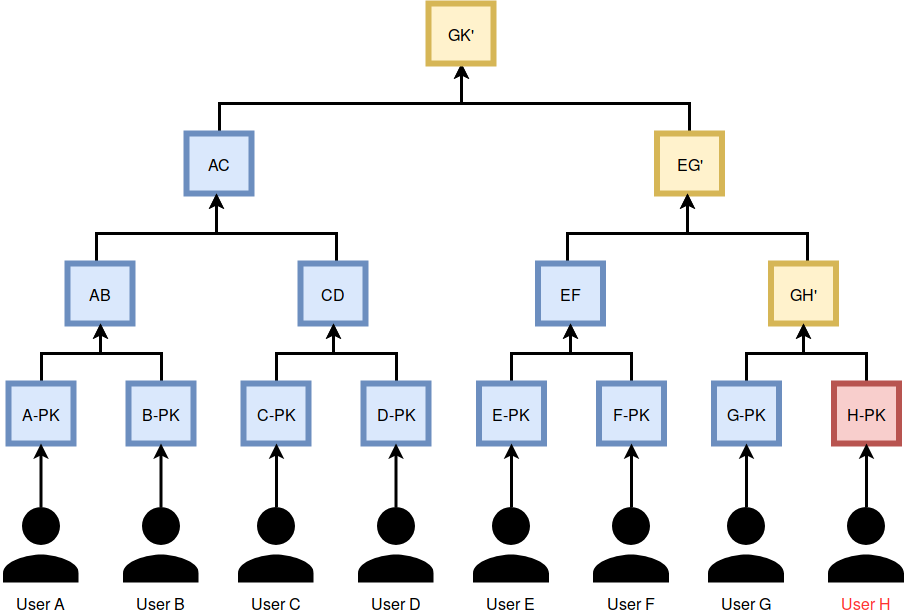
\includegraphics[width=0.8\linewidth]{img/LKH.png}
    \caption{Balanced binary \ac{LKH} and \textbf{User H} joins or leaves the group. Node marked in yellow is newly added to the group. Node marked in green require an update and need to be stored locally by the user.}
    \label{fig:lkh}
\end{figure*}
\todo{fix image placement}

Logical Key Hirachy (\ac{LKH})\cite{wallner1999key} is a \ac{GKMP} that reduces user side storage and rekey-tranmissions by organizing users keys in a tree hirachy and maximaly exploiting the use of multicast messaging. The whole tree is mainted by a central \textit{Key Distribution Center} (\ac{KDC}). In the litrature it is explicitly stated that this trees neither habe to be balanced nor binary, but for the sake of simplity excatly this is assumed. Users (and their respecitv public keys) are organized on the lealf if this tree. Each node is composed of a key that is encrypted respectivly with its children keys. This encrypted key is known to all leafts related to this node and can, on change of this node, be transmitted in one multicast transmission to all its leafs. The root node summarizes the \ac{GK}. The \ac{GK} is used in the same way as in \ac{GKMP} to secure the group communication. 

While in \ac{GKMP} each user needs to store each members public key to eventually rekey the group, in \ac{LKH} each user only needs to store $log(n) +1$ keys (path from leaf to root node). Beginning from the buttom each leaf node could decrypt the next parent node until it arrive at the root node. The other adventage is that many members share the same keys. So it is more efficient to transmit this keys in a multicast setting. \ac{LKH} needs to do $2log(n)$ multicast transmissions and analogous $2log(n)$ encryptions on each member leave or join.  Here each updated key in the path from leaf to root node needs to be updated and encrypted two times: One time with the key of right children node and second with the key of the left children node. 

In figure \ref{fig:lkh} user H recently joined the group which means, that to ensure backward secrecy, the keys in node $GH$, $EG$ and $GK$ must be updated. The key server will choose a new $GH'$, $EG'$ and $GK'$ and encrypts and distributes them in a buttom up fashion starting by $GH'$. $GH'$ is encrypted with user Gs and user Hs public key (G-PK, H-PK) and send to them. Next, user E and F receive in a multicast transmission $EG'$, which is encrypted with EF and user G and H receive in a multicast transmission $EG'$ which is now encrypted with the newly established $GH'$ key. Finally, \ac{GK} needs to be updated. $GK'$ is encrypted with AC to multicast transmit it to the users A, B, C and D. And $GK'$ is encrypted with $EG'$ to transmit it in one message to user E, F, G and H. In the similar fashion a user would be added to the tree. Forward secrecy is implicitly given and not easly to remove from this scheme.

\subsubsection{One-way function trees}
To reduce the transmission and encryption overhead of $2log(n)$ to even further to $log(n)$ other schemes use pheudorandom functions \cite{canetti1999multicast} or one-way functions \cite{sherman2003key} to compute the required keys in the path. This schemes are strongly related to merkel trees, since each update of the user set, will force an update of the root node, the group key.

Each user stores a blinded key for each siblings node in the path to the root node. Starting from the individual key, a user can compute the blinded version of his key. To compute the next parent key, a user uses his blinded key, together with the siblings blinded key, which is feeded into a one way function to create the key for the parent node. This node needs to be blinded to serve as the input for the next level. In such way the user can compute the needed keys up to the GK. 

Lets assume user H joined the group in figure \ref{fig:lkh} and given a crypographically secure hash function $h$. First, user H needs to receive the blinded keys, $h(AC)$, $h(EF)$ and $h(G-PK)$ which he stores locally in addition to his own public key $H-PK$. One-way function trees has the same storage overhead as LKH with $log(n) + 1$.  As already known from LKH, we need to update $GH$, $EG$ and $GK$. This nodes are computed from their children blinded values using a merging function $m$ which takes two inputs and procues one output. This could for example be the concatination of both inputs and then applying $h$ to receive a fixed length output value. Starting from the button,  $GH'$ is computed as $m(f(G-PK), f(G-PK))$, analogous $EG' = m(f(EF), f(GH'))$ and finally the updated group key $GK' = m(f(AG), f(EG')$. The new blinded keys are distributed to their respective users using multicast transmissiong, reducing the transmission and encryption overhead to $log(n)$. Again backward secrecy is implicitly given by the natural update process of each node.


\subsubsection{Comparison}
\todo{find better title}  

\begin{table*}[!ht]
\centering
\begin{tabular}{l 		| l 						| l 							| l 						| l 						| l }
 						& \textbf{Bdrive}			& \textbf{\ac{GKMP}}					& \textbf{\ac{LKH}}				& \textbf{\ac{OWFT}} 			& \textbf{\ac{GDH}.1}\\
\hline
\textbf{inizial share} 																																		\\
keys 					& $nf$	 					& $1$  							& $n-1$  					& $n$	 					& $1$ 			\\
messages (unicast)		& $nf$	  					& $n$ 							& $n(log_2(n) + 1)$ 		& $2n(log_2(n) + 1)$		& $2(n - 1)$	\\
messages (multicast) 	& $nf$	 					& $n$ 							& $log_2(n) + 1$ 			& $n - 2$ 					& $2(n - 1)$ 	\\
encryptions				& $nf$	 					& $f + n$ 						& $f + n -1$				& $f + n -1$				& $f + n$		\\
\hline
\textbf{member join} 																																		\\
keys 					& $f$   					& $1$  							& $3 log_2(n)$				& $log_2(n)$				& $1$			\\
messages (unicast)		& $f$  						& $1$			 				& $2(n - 1)$				& $n$  						& $2(n - 1)$	\\
messages (multicast) 	& $f$ 	 					& $1$ 		 					& $2 log_2(n)$				& $log_2(n)$				& $2(n - 1)$	\\
encryptions				& $f$  						& $f + 1$		 				& $f + 2(log_2(n))$ 		& $f + log_2(n)$			& $f + 2$	 	\\
\hline
\textbf{member leave}																																		\\
keys 					& $0$						& $1$			  				& $3 log_2(n)$				& $log_2(n)$				& $1$			\\
messages (unicast)		& $0$						& $n$			 				& $2(n - 1)$ 				& $0$	  					& $2(n-1)$		\\
messages (multicast)	& $0$						& $n$			 				& $2 log_2(n)$				& $log_2(n)$				& $2(n-1)$		\\ 
encryptions 			& $0$						& $f + n$ 						& $f + 2 (log_2(n))$ 		& $f + log_2(n)$	 		& $f+n$			\\
\hline	
\textbf{addition of filekey}																																\\
keys 					& $n$		 				& $0$							& $0$	 					& $0$		 				& $0$			\\
messages (unicast)		& $n$		 				& $0$	 						& $0$ 						& $0$		 				& $0$			\\
messages (multicast)	& $n$ 						& $0$ 							& $0$ 						& $0$	 					& $0$			\\
encryptions				& $n$ 						& $1$ 							& $1$ 						& $1$		 				& $1$			\\
\hline
\end{tabular}
\caption{Comparison of secure group communication schemes. $n$ donates the number of members, $f$ the number of file keys. Backward secrecy is ensured in each scheme. Assuming a balanced binary tree as in figure \ref{fig:lkh}}
\label{tab:comparisons}
\end{table*}

The following table will compare the discussed schemes against each other regarding number of keys, messages, and ecnryptions on inizialisation of the group, when a member joins or leaves and on addition of a new file. 

It is assumped that clients already downloaded the public keys of their desired group members. Backward secrecy need to be ensured every time a member leaves the group.
Further, messages in table \ref{tab:comparisons} are transmissions that contain a key. There are also meta messages that nodify the members about a new file upload or the removal of a member, etc. They are left out since they add a contant overhead to all schemes.  If a message could be processed by multible communication partners we only need to send the message once, in a multicast transmission.

Some cloud clearly see that Bdrives scheme is not optimal at all compared to the different approaches. In fact Bdrive has the worst perforamnce on inizialisation, addition of a filekey and on average also on member join. In general we can assume that $f > n$ since people tend to have more files then members in a share. However, Bdrive has great performance on member leave since client simply don't encrypt anymore for the left member.

It is hard to extract a clear winner. Each of the schemes have their own strength and weaknesses. \ac{GKMP} has the best inizialisation overhead and \ac{OWFT} the best rekeying overhead. We can clearly extract from the table that all secure group schmes perform better on filekey upload. Bdrive needs to distribute the new key encryption filekey to $n$ devices. On the other hand the \ac{GK} only needs to encrypt the filekey once. Automatically all members have access to the new filekey. 

Under the assumption that do not need backward secrey, we select \ac{GKMP} the most performant candidate. It has great inizialisation overhead is easily understandable and profits from the fact that we do not need backward secrey on member join. \ac{LKH} and \ac{OWFT} both do not get better performance if we remove the backward secrecy constain since this security feature is deeply implemetned in the design of thouse schemes. 